\documentclass{beamer}
\usepackage[utf8]{inputenc}
\usepackage{utopia} %font utopia imported
\usepackage[normalem]{ulem}
\usepackage{listings}
\usepackage{amsmath}
\usepackage{tikz}
\usetikzlibrary{arrows.meta, calc, matrix} % <-- added library
\usepackage{graphicx}
\graphicspath{{C:/Users/marco/Documents/DocumentosLatex/}}


\usetheme{madrid}
\usecolortheme{default}

\lstdefinestyle{mystyle}{
	backgroundcolor=\color{white},   
	commentstyle=\color{green},
	keywordstyle=\color{blue},
	numberstyle=\tiny\color{gray},
	stringstyle=\color{cyan},
	basicstyle=\ttfamily\footnotesize,
	breakatwhitespace=false,         
	breaklines=true,                 
	captionpos=b,                    
	keepspaces=true,                 
	numbers= none,                    
	numbersep=5pt,                  
	showspaces=false,                
	showstringspaces=false,
	showtabs=false,                  
	tabsize=2
}

\lstset{style = mystyle}

%------------------------------------------------------------
%This block of code defines the information to appear in the
%Title page
\title[Ordenación por distribución] %optional
{Ordenación por distribución}

\subtitle{Cómo ordenar con coste lineal}

\author[Marcos Herrero] % (optional)
{Marcos Herrero Agustín}


\date[] % (optional)
{}



%End of title page configuration block
%------------------------------------------------------------



%------------------------------------------------------------
%The next block of commands puts the table of contents at the 
%beginning of each section and highlights the current section:

\AtBeginSection[]
{
	\begin{frame}
	\frametitle{Table of Contents}
	\tableofcontents[currentsection]
\end{frame}
}
%------------------------------------------------------------


\begin{document}

%The next statement creates the title page.
\frame{\titlepage}


%---------------------------------------------------------
%This block of code is for the table of contents after
%the title page
\begin{frame}
\frametitle{Contenidos}
\tableofcontents
\end{frame}
%---------------------------------------------------------


\section{Motivación}

\begin{frame}
\frametitle{Costes de algoritmos de ordenación vistos hasta ahora}
\begin{tabular}{|c|c|c|c|}
	\hline
	Algoritmo & Caso peor & Caso promedio & Espacio adicional\\
	\hline
	Bubble Sort& $O(n^2)$ & $O(n^2)$ & $O(1)$ \\
	Selection Sort & $O(n^2)$ & $O(n^2)$ & $O(1)$ \\
	Insertion Sort & $O(n^2)$ & $O(n^2)$ & $O(1)$ \\
	Quicksort & $O(n^2)$ & $O(n\log n)$ & $O(n)$ \\
	Mergesort & $O(n\log n)$ & $O(n\log n)$ & $O(n)$ \\
	Heapsort & $O(n\log n)$ & $O(n\log n)$ & $O(1)$ \\
	\hline
\end{tabular}

\vspace{1cm}
\alert{¿Lo podemos hacer mejor?}
\end{frame}

\begin{frame}
\frametitle{Árboles de decisión}
Dado un algoritmo de ordenación basado en comparaciones, un \alert{árbol de decisión} de tamaño $n$ es un árbol binario que representa todas las posibles secuencias de comparaciones que realizaría el algoritmo para llegar a la solución desde una entrada arbitraria de tamaño $n$. La ejecución del algoritmo para una entrada concreta correspondería a trazar un camino en el árbol desde la raíz hasta una de las hojas.

Por ejemplo, para un tamaño de entrada $3$ el siguiente árbol de decisión representa el algoritmo de ordenación por inserción:

\centering
\scriptsize
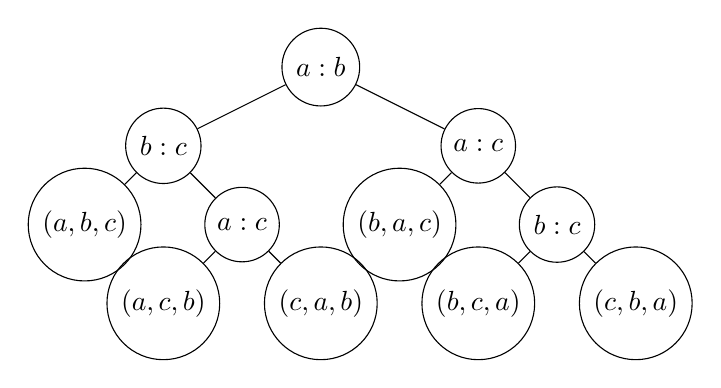
\begin{tikzpicture}
\node[circle, draw] (1) at (0,0) {$a:b$};
\node[circle, draw] (2) at (-2,-1) {$b:c$};
\node[circle, draw] (3) at (-3,-2) {$(a,b,c)$};
\node[circle, draw] (4) at (-1,-2) {$a:c$};
\node[circle, draw] (5) at (-2,-3) {$(a,c,b)$};
\node[circle, draw] (6) at (0,-3) {$(c,a,b)$};
\node[circle, draw] (7) at (2,-1) {$a:c$};
\node[circle, draw] (8) at (1,-2) {$(b,a,c)$};
\node[circle, draw] (9) at (3,-2) {$b:c$};
\node[circle, draw] (10) at (2,-3) {$(b,c,a)$};
\node[circle, draw] (11) at (4,-3) {$(c,b,a)$};
\draw (1)--(2)--(3);
\draw (2)--(4)--(5);
\draw (4)--(6);
\draw (1)--(7)--(8);
\draw (7)--(9)--(10);
\draw (9)--(11);
\end{tikzpicture}
\end{frame}

\begin{frame}
\begin{block}{Teorema}
	Todo algoritmo de ordenación basado en comparaciones tiene coste en $\Omega(n\log n)$ en el caso peor
\end{block}

\begin{itemize}
	\item[Dem] Sea $n$ el tamaño de la entrada. Todo algoritmo de ordenación basado en comparaciones puede representarse como un árbol de decisión, en el que las $l$ hojas representan posibles permutaciones de la entrada. Como todas las permutaciones de la entrada han de estar en el árbol, $n! \leq l$. En el caso peor, el algoritmo realiza tantas comparaciones como la altura $h$ del árbol. Como se trata de un árbol binario , se tiene:
	$$n!\leq l\leq 2^h$$
	y esto implica
	$$h \geq \log(n!)= \sum_{i=2}^n\log(i) \geq\int_1^n \log x dx = \frac1{ln2}(n\ln n-n+1)$$
\end{itemize}
\end{frame}

\begin{frame}
\begin{itemize}
\item[]$$\geq n \log n-1.45n\approx n\log n$$
Por tanto, todo algoritmo de ordenación basado en comparaciones realiza, en el caso peor, un número de comparaciones en el orden de $n\log n$
\end{itemize}
\vspace{1cm}
Se puede probar un resultado similar para el coste en el caso promedio. Como consecuencia, obtenemos que Mergesort y Quicksort son óptimos como algoritmos de ordenación basados en comparaciones entre claves. 

Vamos  ver, sin embargo, que existen otros procedimientos de ordenación no basados en comparaciones y que permiten obtener algoritmos más rápidos, estableciendo ciertas restricciones sobre la entrada.
\end{frame}



\section{Counting Sort}


%---------------------------------------------------------
%Highlighting text
\begin{frame}
\alert{Counting Sort} es un algoritmo sencillo que permite ordenar de  forma rápida un vector de $n$ objetos cuyas claves toman valores en un conjunto ordenado $\mathcal{F}$ de pocos elementos.
\begin{itemize}
	\item Identificando cada clave con un número natural, supondremos que $\mathcal{F}= \{0,...,k-1\}$ 
\end{itemize}

La idea del algoritmo se basa en recorrer el conjunto de claves posibles (los enteros de $0$ a $k-1$) y determinar, para cada una, la posición o posiciones del vector en que deberán situarse los elementos con dicha clave.
\begin{block}{Observación} 
No se realizan comparaciones entre las claves de los elementos a ordenar, así que el coste en el caso peor de este algoritmo no tiene por qué estar acotado inferiormente por $n \log n$. 
\end{block}

\end{frame}
%---------------------------------------------------------

\begin{frame}
\frametitle{Algoritmo}
Vamos a ver el proceso que sigue con un ejemplo:
\begin{itemize}
	\item[1] Comenzamos contando el número de apariciones de cada clave, llevando la cuenta en un vector de $k$ posiciones. 
\end{itemize}

\begin{columns}
	\column{0.3\textwidth}
	\raggedleft
	
	\vspace{1 cm}
	v
	
	\vspace{2 cm}
	count
	
	\column{0.7 \textwidth}
	
	 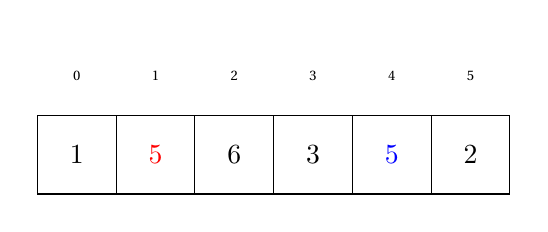
\begin{tikzpicture} [nodes in empty cells,
	nodes={minimum width=1cm, minimum height=1cm},
	row sep=-\pgflinewidth, column sep=-\pgflinewidth]
	%   border/.style={draw}
	
	\matrix(vector)[matrix of nodes, ampersand replacement=\&, % <- added ampersand replacement
	row 1/.style={nodes={draw=none, minimum width=0.3cm}},
	nodes={draw}]
	{ % use \& instead of & as column separator
		\tiny{0} \& \tiny{1} \& \tiny{2} \& \tiny{3} \& \tiny{4} \& \tiny{5}\\
		$1$ \& $\color{red}5$ \& $6$ \& $3$ \& $\color{blue}5$ \& $2$\\
	};
	
	
	\end{tikzpicture}
	
	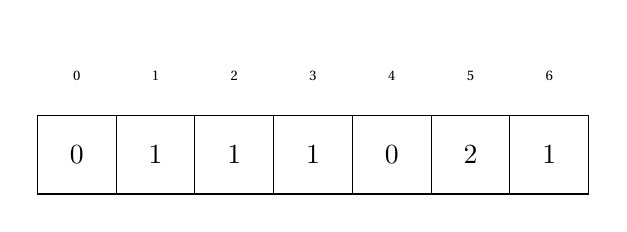
\begin{tikzpicture} [nodes in empty cells,
	nodes={minimum width=1cm, minimum height=1cm},
	row sep=-\pgflinewidth, column sep=-\pgflinewidth]
	%    border/.style={draw}
	
	\matrix(vector)[matrix of nodes, ampersand replacement=\&, % <- added ampersand replacement
	row 1/.style={nodes={draw=none, minimum width=0.3cm}},
	nodes={draw}]
	{ % use \& instead of & as column separator
		\tiny{0} \& \tiny{1} \& \tiny{2} \& \tiny{3} \& \tiny{4} \& \tiny{5} \& \tiny{6}\\
		$0$ \& $1$ \& $1$ \& $1$ \& $0$ \& $2$ \& $1$\\
	};
	
	\end{tikzpicture}
	
\end{columns}	

\end{frame}

\begin{frame}

\begin{itemize}
	\item[2] A continuación, recorremos este vector, calculando en qué rango de posiciones  debería ir cada una de las claves.
\end{itemize}

\begin{columns}
	\column{0.3\textwidth}
	\raggedleft
	
	\vspace{1 cm}
	v
	
	\vspace{2 cm}
	count
	
	\vspace{2 cm}
	pos
	\column{0.7 \textwidth}
	
	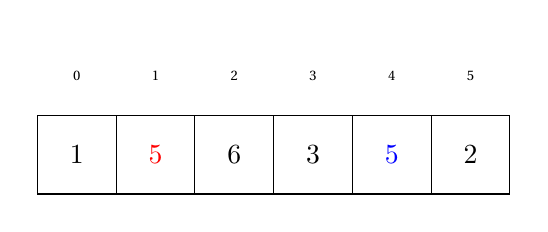
\begin{tikzpicture} [nodes in empty cells,
	nodes={minimum width=1cm, minimum height=1cm},
	row sep=-\pgflinewidth, column sep=-\pgflinewidth]
	%   border/.style={draw}
	
	\matrix(vector)[matrix of nodes, ampersand replacement=\&, % <- added ampersand replacement
	row 1/.style={nodes={draw=none, minimum width=0.3cm}},
	nodes={draw}]
	{ % use \& instead of & as column separator
		\tiny{0} \& \tiny{1} \& \tiny{2} \& \tiny{3} \& \tiny{4} \& \tiny{5}\\
		$1$ \& $\color{red}5$ \& $6$ \& $3$ \& $\color{blue}5$ \& $2$\\
	};
	
	
	\end{tikzpicture}

	
	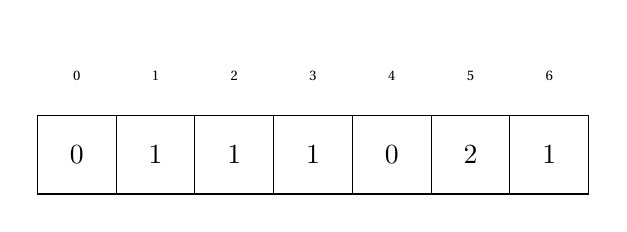
\begin{tikzpicture} [nodes in empty cells,
	nodes={minimum width=1cm, minimum height=1cm},
	row sep=-\pgflinewidth, column sep=-\pgflinewidth]
	%    border/.style={draw}
	
	\matrix(vector)[matrix of nodes, ampersand replacement=\&, % <- added ampersand replacement
	row 1/.style={nodes={draw=none, minimum width=0.3cm}},
	nodes={draw}]
	{ % use \& instead of & as column separator
		\tiny{0} \& \tiny{1} \& \tiny{2} \& \tiny{3} \& \tiny{4} \& \tiny{5} \& \tiny{6}\\
		$0$ \& $1$ \& $1$ \& $1$ \& $0$ \& $2$ \& $1$\\
	};
	
	\end{tikzpicture}
	
	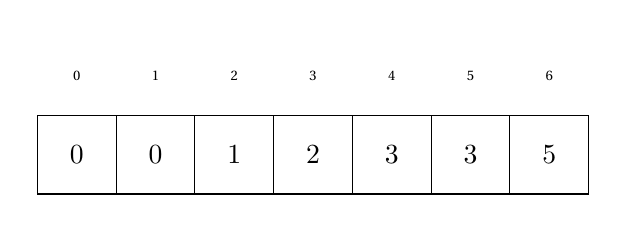
\begin{tikzpicture} [nodes in empty cells,
	nodes={minimum width=1cm, minimum height=1cm},
	row sep=-\pgflinewidth, column sep=-\pgflinewidth]
	%    border/.style={draw}
	
	\matrix(vector)[matrix of nodes, ampersand replacement=\&, % <- added ampersand replacement
	row 1/.style={nodes={draw=none, minimum width=0.3cm}},
	nodes={draw}]
	{ % use \& instead of & as column separator
		\tiny{0} \& \tiny{1} \& \tiny{2} \& \tiny{3} \& \tiny{4} \& \tiny{5} \& \tiny{6}\\
		$0$ \& $0$ \& $1$ \& $2$ \& $3$ \& $3$ \& $5$\\
	};
	
	\end{tikzpicture}
	
\end{columns}	

\end{frame}

\begin{frame}

\begin{itemize}
	\item[3] Por último, recorriendo nuevamente el vector inicial colocamos cada elemento en la posición que corresponde según su clave.
\end{itemize}

\begin{columns}
	\column{0.3\textwidth}
	\raggedleft
	
	\vspace{1 cm}
	v
	
	\vspace{2 cm}
	pos
	
	\vspace{2 cm}
	w(v ordenado)
	\column{0.7 \textwidth}
	
	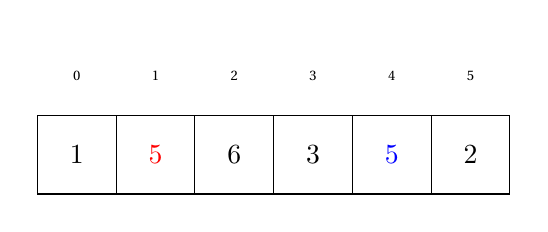
\begin{tikzpicture} [nodes in empty cells,
	nodes={minimum width=1cm, minimum height=1cm},
	row sep=-\pgflinewidth, column sep=-\pgflinewidth]
	%   border/.style={draw}
	
	\matrix(vector)[matrix of nodes, ampersand replacement=\&, % <- added ampersand replacement
	row 1/.style={nodes={draw=none, minimum width=0.3cm}},
	nodes={draw}]
	{ % use \& instead of & as column separator
		\tiny{0} \& \tiny{1} \& \tiny{2} \& \tiny{3} \& \tiny{4} \& \tiny{5}\\
		$1$ \& $\color{red}5$ \& $6$ \& $3$ \& $\color{blue}5$ \& $2$\\
	};
	
	
	\end{tikzpicture}
	
	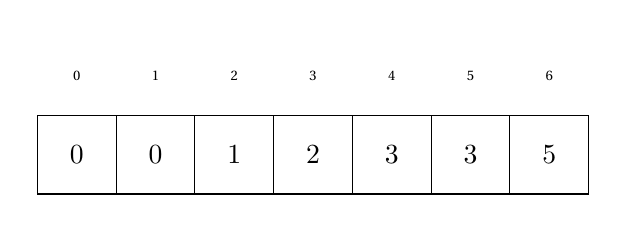
\begin{tikzpicture} [nodes in empty cells,
	nodes={minimum width=1cm, minimum height=1cm},
	row sep=-\pgflinewidth, column sep=-\pgflinewidth]
	%    border/.style={draw}
	
	\matrix(vector)[matrix of nodes, ampersand replacement=\&, % <- added ampersand replacement
	row 1/.style={nodes={draw=none, minimum width=0.3cm}},
	nodes={draw}]
	{ % use \& instead of & as column separator
		\tiny{0} \& \tiny{1} \& \tiny{2} \& \tiny{3} \& \tiny{4} \& \tiny{5} \& \tiny{6}\\
		$0$ \& $0$ \& $1$ \& $2$ \& $3$ \& $3$ \& $5$\\
	};
	
	
	\end{tikzpicture}
	
	\begin{tikzpicture} [nodes in empty cells,
	nodes={minimum width=1cm, minimum height=1cm},
	row sep=-\pgflinewidth, column sep=-\pgflinewidth]
	%    border/.style={draw}
	
	\matrix(vector)[matrix of nodes, ampersand replacement=\&, % <- added ampersand replacement
	row 1/.style={nodes={draw=none, minimum width=0.3cm}},
	nodes={draw}]
	{ % use \& instead of & as column separator
		\tiny{0} \& \tiny{1} \& \tiny{2} \& \tiny{3} \& \tiny{4} \& \tiny{5}\\
		$$ \& $$ \& $$ \& $$ \& $$ \& $$ \& $$\\
	};

	\end{tikzpicture}
	
\end{columns}
\end{frame}

\begin{frame}

\begin{itemize}
	\item[3] Por último, recorriendo nuevamente el vector inicial colocamos cada elemento en la posición que corresponde según su clave.
\end{itemize}

\begin{columns}
	\column{0.3\textwidth}
	\raggedleft
	
	\vspace{1 cm}
	v
	
	\vspace{2 cm}
	pos
	
	\vspace{2 cm}
	w(v ordenado)
	\column{0.7 \textwidth}
	
	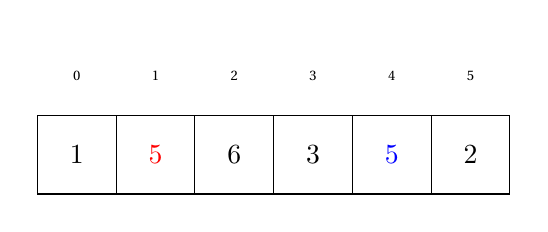
\begin{tikzpicture} [nodes in empty cells,
	nodes={minimum width=1cm, minimum height=1cm},
	row sep=-\pgflinewidth, column sep=-\pgflinewidth]
	%   border/.style={draw}
	
	\matrix(vector)[matrix of nodes, ampersand replacement=\&, % <- added ampersand replacement
	row 1/.style={nodes={draw=none, minimum width=0.3cm}},
	nodes={draw}]
	{ % use \& instead of & as column separator
		\tiny{0} \& \tiny{1} \& \tiny{2} \& \tiny{3} \& \tiny{4} \& \tiny{5}\\
		$1$ \& $\color{red}5$ \& $6$ \& $3$ \& $\color{blue}5$ \& $2$\\
	};
	
	
	\end{tikzpicture}
	
	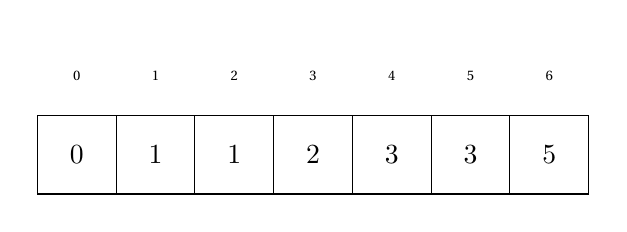
\begin{tikzpicture} [nodes in empty cells,
	nodes={minimum width=1cm, minimum height=1cm},
	row sep=-\pgflinewidth, column sep=-\pgflinewidth]
	%    border/.style={draw}
	
	\matrix(vector)[matrix of nodes, ampersand replacement=\&, % <- added ampersand replacement
	row 1/.style={nodes={draw=none, minimum width=0.3cm}},
	nodes={draw}]
	{ % use \& instead of & as column separator
		\tiny{0} \& \tiny{1} \& \tiny{2} \& \tiny{3} \& \tiny{4} \& \tiny{5} \& \tiny{6}\\
		$0$ \& $1$ \& $1$ \& $2$ \& $3$ \& $3$ \& $5$\\
	};
	
	
	\end{tikzpicture}
	
	\begin{tikzpicture} [nodes in empty cells,
	nodes={minimum width=1cm, minimum height=1cm},
	row sep=-\pgflinewidth, column sep=-\pgflinewidth]
	%    border/.style={draw}
	
	\matrix(vector)[matrix of nodes, ampersand replacement=\&, % <- added ampersand replacement
	row 1/.style={nodes={draw=none, minimum width=0.3cm}},
	nodes={draw}]
	{ % use \& instead of & as column separator
		\tiny{0} \& \tiny{1} \& \tiny{2} \& \tiny{3} \& \tiny{4} \& \tiny{5}\\
		$1$ \& $$ \& $$ \& $$ \& $$ \& $$\\
	};
	
	\end{tikzpicture}
	
\end{columns}
\end{frame}

\begin{frame}

\begin{itemize}
	\item[3] Por último, recorriendo nuevamente el vector inicial colocamos cada elemento en la posición que corresponde según su clave.
\end{itemize}

\begin{columns}
	\column{0.3\textwidth}
	\raggedleft
	
	\vspace{1 cm}
	v
	
	\vspace{2 cm}
	pos
	
	\vspace{2 cm}
	w(v ordenado)
	\column{0.7 \textwidth}
	
	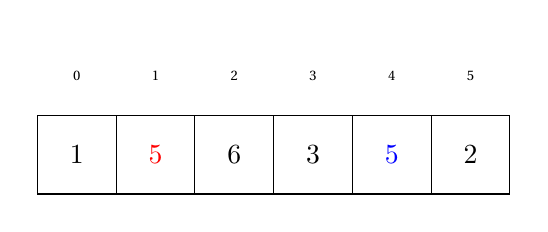
\begin{tikzpicture} [nodes in empty cells,
	nodes={minimum width=1cm, minimum height=1cm},
	row sep=-\pgflinewidth, column sep=-\pgflinewidth]
	%   border/.style={draw}
	
	\matrix(vector)[matrix of nodes, ampersand replacement=\&, % <- added ampersand replacement
	row 1/.style={nodes={draw=none, minimum width=0.3cm}},
	nodes={draw}]
	{ % use \& instead of & as column separator
		\tiny{0} \& \tiny{1} \& \tiny{2} \& \tiny{3} \& \tiny{4} \& \tiny{5}\\
		$1$ \& $\color{red}5$ \& $6$ \& $3$ \& $\color{blue}5$ \& $2$\\
	};
	
	
	\end{tikzpicture}
	
	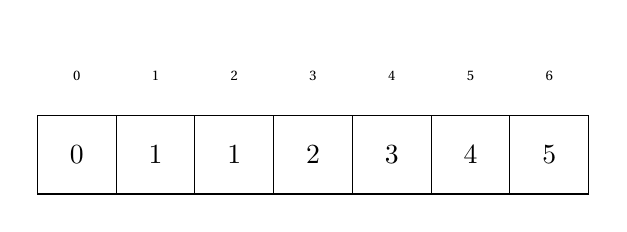
\begin{tikzpicture} [nodes in empty cells,
	nodes={minimum width=1cm, minimum height=1cm},
	row sep=-\pgflinewidth, column sep=-\pgflinewidth]
	%    border/.style={draw}
	
	\matrix(vector)[matrix of nodes, ampersand replacement=\&, % <- added ampersand replacement
	row 1/.style={nodes={draw=none, minimum width=0.3cm}},
	nodes={draw}]
	{ % use \& instead of & as column separator
		\tiny{0} \& \tiny{1} \& \tiny{2} \& \tiny{3} \& \tiny{4} \& \tiny{5} \& \tiny{6}\\
		$0$ \& $1$ \& $1$ \& $2$ \& $3$ \& $4$ \& $5$\\
	};
	
	
	\end{tikzpicture}
	
	\begin{tikzpicture} [nodes in empty cells,
	nodes={minimum width=1cm, minimum height=1cm},
	row sep=-\pgflinewidth, column sep=-\pgflinewidth]
	%    border/.style={draw}
	
	\matrix(vector)[matrix of nodes, ampersand replacement=\&, % <- added ampersand replacement
	row 1/.style={nodes={draw=none, minimum width=0.3cm}},
	nodes={draw}]
	{ % use \& instead of & as column separator
		\tiny{0} \& \tiny{1} \& \tiny{2} \& \tiny{3} \& \tiny{4} \& \tiny{5}\\
		$1$ \& $$ \& $$ \& $\color{red}5$ \& $$ \& $$ \\
	};
	
	\end{tikzpicture}
	
\end{columns}
\end{frame}

\begin{frame}

\begin{itemize}
\item[3] Por último, recorriendo nuevamente el vector inicial colocamos cada elemento en la posición que corresponde según su clave.
\end{itemize}

\begin{columns}
\column{0.3\textwidth}
\raggedleft

\vspace{1 cm}
v

\vspace{2 cm}
pos

\vspace{2 cm}
w(v ordenado)
\column{0.7 \textwidth}

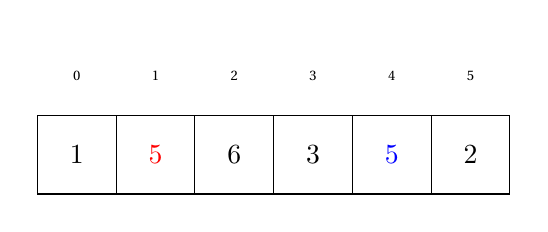
\begin{tikzpicture} [nodes in empty cells,
nodes={minimum width=1cm, minimum height=1cm},
row sep=-\pgflinewidth, column sep=-\pgflinewidth]
%   border/.style={draw}

\matrix(vector)[matrix of nodes, ampersand replacement=\&, % <- added ampersand replacement
row 1/.style={nodes={draw=none, minimum width=0.3cm}},
nodes={draw}]
{ % use \& instead of & as column separator
	\tiny{0} \& \tiny{1} \& \tiny{2} \& \tiny{3} \& \tiny{4} \& \tiny{5}\\
	$1$ \& $\color{red}5$ \& $6$ \& $3$ \& $\color{blue}5$ \& $2$\\
};


\end{tikzpicture}

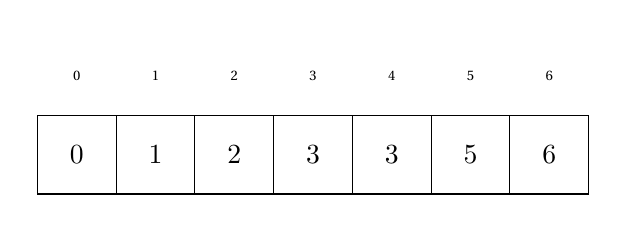
\begin{tikzpicture} [nodes in empty cells,
nodes={minimum width=1cm, minimum height=1cm},
row sep=-\pgflinewidth, column sep=-\pgflinewidth]
%    border/.style={draw}

\matrix(vector)[matrix of nodes, ampersand replacement=\&, % <- added ampersand replacement
row 1/.style={nodes={draw=none, minimum width=0.3cm}},
nodes={draw}]
{ % use \& instead of & as column separator
	\tiny{0} \& \tiny{1} \& \tiny{2} \& \tiny{3} \& \tiny{4} \& \tiny{5} \& \tiny{6}\\
	$0$ \& $1$ \& $2$ \& $3$ \& $3$ \& $5$ \& $6$\\
};


\end{tikzpicture}

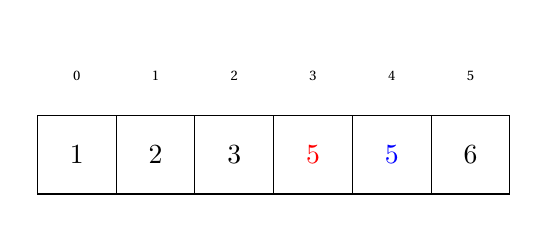
\begin{tikzpicture} [nodes in empty cells,
nodes={minimum width=1cm, minimum height=1cm},
row sep=-\pgflinewidth, column sep=-\pgflinewidth]
%    border/.style={draw}

\matrix(vector)[matrix of nodes, ampersand replacement=\&, % <- added ampersand replacement
row 1/.style={nodes={draw=none, minimum width=0.3cm}},
nodes={draw}]
{ % use \& instead of & as column separator
	\tiny{0} \& \tiny{1} \& \tiny{2} \& \tiny{3} \& \tiny{4} \& \tiny{5}\\
	$1$ \& $2$ \& $3$ \& $\color{red}5$ \& $\color{blue}5$ \& $6$ \\
};

\end{tikzpicture}

\end{columns}
\end{frame}

\begin{frame}[fragile]
\frametitle{Código}
\begin{columns}
	\column{0.95\textwidth}
	
	\begin{lstlisting}[language = C++, basicstyle=\ttfamily\scriptsize]
	void countingSort(std::vector<int> & v, int k) { 
	  int n = v.size();
	  std::vector<int> count(k, 0);
	
	  for (int i = 0; i < n;  ++i) ++count[v[i]];
	
	  int empieza = 0, aux;
	  for (int i = 0; i < k; ++i) {
	    aux = count[i] + empieza;   
	    count[i] = empieza;         
	    empieza = aux;
	  }
	
	  std::vector<int> w(n);
	  for (int i = 0; i < n; ++i) {
 	    w[count[v[i]]] = v[i];     
	    ++count[v[i]];           
	  }
	
	  v = std::move(w);
	}
	\end{lstlisting}
	
	\column{0.05\textwidth}
	
	\vspace{1.7 cm}
	
	$O(n)$
	\vspace{1 cm}
	
	$O(k)$
	\vspace{1.5 cm}
	
	$O(n)$
	\vspace{2 cm}
\end{columns}

\end{frame}

%---------------------------------------------------------
\begin{frame}
\frametitle{Análisis de la complejidad}
Para un vector de $n$ elementos y claves acotadas por $k$, el algoritmo tiene coste en tiempo $O(n+k)$. Por tanto, si $k\in O(n)$ este es un algoritmo de coste lineal sobre el número de elementos del vector.

\vspace{0.5 cm}
El coste en espacio adicional está también en $O(n+k)$ debido a que se requiere almacenar el vector de cuentas y no se ordena sobre el propio vector de entrada, sino en un vector nuevo.




\end{frame}
%---------------------------------------------------------

\begin{frame}
 \frametitle{Estabilidad}
 
  Es importante notar que, cuando coinciden las claves, Counting Sort respeta el orden inicial de los elementos , es decir, se trata un \alert{algoritmo de ordenación estable}. Esta propiedad es clave para algunas de las aplicaciones de este algoritmo, como su uso auxiliar en RadixSort.
  
  
  \begin{columns}
  	\column{0.3\textwidth}
  	\raggedleft
  	
  	\vspace{1 cm}
  	v
  	
  	\vspace{2 cm}
  	w(v ordenado)
  	\column{0.7 \textwidth}
  	
  	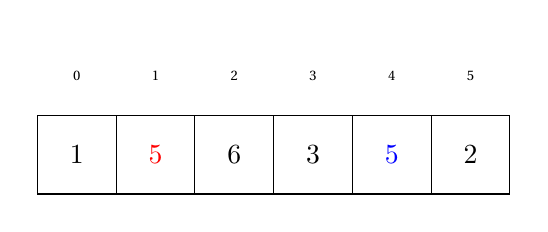
\begin{tikzpicture} [nodes in empty cells,
  	nodes={minimum width=1cm, minimum height=1cm},
  	row sep=-\pgflinewidth, column sep=-\pgflinewidth]
  	%   border/.style={draw}
  	
  	\matrix(vector)[matrix of nodes, ampersand replacement=\&, % <- added ampersand replacement
  	row 1/.style={nodes={draw=none, minimum width=0.3cm}},
  	nodes={draw}]
  	{ % use \& instead of & as column separator
  		\tiny{0} \& \tiny{1} \& \tiny{2} \& \tiny{3} \& \tiny{4} \& \tiny{5}\\
  		$1$ \& $\color{red}5$ \& $6$ \& $3$ \& $\color{blue}5$ \& $2$\\
  	};
  	
  	
  	\end{tikzpicture}
  	
  	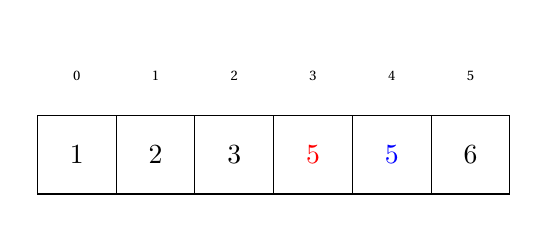
\begin{tikzpicture} [nodes in empty cells,
  	nodes={minimum width=1cm, minimum height=1cm},
  	row sep=-\pgflinewidth, column sep=-\pgflinewidth]
  	%    border/.style={draw}
  	
  	\matrix(vector)[matrix of nodes, ampersand replacement=\&, % <- added ampersand replacement
  	row 1/.style={nodes={draw=none, minimum width=0.3cm}},
  	nodes={draw}]
  	{ % use \& instead of & as column separator
  		\tiny{0} \& \tiny{1} \& \tiny{2} \& \tiny{3} \& \tiny{4} \& \tiny{5}\\
  		$1$ \& $2$ \& $3$ \& $\color{red}5$ \& $\color{blue}5$ \& $6$ \\
  	};
  	
  	\end{tikzpicture}
  	
  \end{columns}
  
\end{frame}

\section{Radix Sort}

\begin{frame}
  \alert{RadixSort} es un algoritmo de ordenación lexicográfica.
  \begin{itemize}
  	\item Se aplica sobre conjuntos de elementos cuyas claves pueden verse como secuencias de \alert{dígitos} (números, palabras,...), que toman valores en un conjunto finito ordenado.
  	\item Dado un problema de este tipo, llamamos \alert{alfabeto} al conjunto finito de valores que pueden tomar los dígitos de las secuencias. Denotamos por $n$ el número de elementos a ordenar y por $k$ el tamaño del alfabeto.
  	\item Denotamos por $d$ la longitud de la secuencia más larga a ordenar. Rellenando por la izquierda con el dígito de menor valor considerado, puede suponerse que todas las claves de los elementos a ordenar tienen la misma longitud $d$.
  \end{itemize}
\end{frame}

\begin{frame}
 \frametitle{MSDRadixSort}
 \begin{itemize}
 	\item La idea del algoritmo consiste en ordenar todos los elementos según el dígito más significativo, a continuación resolver todos los empates de la iteración anterior utilizando el siguiente dígito, y proseguir así sucesivamente hasta haber considerado los $d$ dígitos de cada secuencia o hasta haber clasificado todos los elementos sin encontrar empates.
 	\item  Al considerar los dígitos de más a menos significativo, la única manera de no perder el trabajo anterior al ordenar por el siguiente dígito es mantener separadas las secuencias que ya fueron diferenciadas por un dígito anterior hasta haber considerado todos los dígitos.
 \end{itemize}
 El esquema del algoritmo es el siguiente:
 \begin{itemize}
 	\item [1] Clasificar los elementos en $k$ cajas(\alert{buckets}) según el valor del dígito más significativo
 	\item[2] Ordenar recursivamente cada caja en base a los dígitos sucesivos
 	\item[3] Trasladar ordenadamente el contenido de las cajas al vector final
 \end{itemize}
\end{frame}

\begin{frame}
\frametitle{Ejemplo}
\includegraphics[scale=0.5]{MSDRadixSort}
\end{frame}

\begin{frame}[fragile]
\frametitle{Código}
 \begin{lstlisting}[language = C++, basicstyle=\ttfamily\scriptsize]
const int k = 10;
void MSDradixSort(std::vector<std::string> & v, int d){
  int n = v.size();
  if (n > 1 && d > 0) {
    std::vector<std::vector<std::string>> digitos(k);
    for (int i = 0; i < n; ++i) {
      if (v[i].size() < d) digitos[0].push_back(v[i]);
      else digitos[int(v[i][v[i].size() - d]) - int('0')].push_back(v[i]);
    }

    int ind = 0;
    for (int i = 0; i < k; ++i) {
      MSDradixSort(digitos[i], d - 1); 

      for (int j = 0; j < digitos[i].size(); ++j) {
        v[ind] = digitos[i][j];
        ++ind;
      }

    }
  }
}
\end{lstlisting}
\end{frame}

\begin{frame}
\frametitle{Análisis del coste}
\begin{itemize}
	\item Se tiene un coste en $\Theta(n*d+k^d)$ en el caso peor en que en cada llamada se hacen $k$ llamadas recursivas y la profundidad de todas ellas es de $d$. Además el coste en espacio adicional es $\Theta(n*d)$, debido a que se han de mantener todas los buckets de las llamadas precedentes hasta el final.
	\item Estos costes asintóticos resultan inadmisibles, y nos llevan a afrontar este problema desde otro punto de vista.
\end{itemize}
\end{frame}

\begin{frame}
\frametitle{LSDRadixSort}
\begin{itemize}
	\item El problema del algoritmo anterior radica en que el trabajo a realizar para no perder la ordenación según los dígitos anteriores resulta excesivo. Nos gustaría poder ordenar sucesivamente sobre el vector inicial sin preocuparnos de perder el trabajo anterior.
	\item Esto puede conseguirse planteando el problema a la inversa: comenzando a ordenar por el dígito menos significativo. De esta manera (dejando el trabajo importante para el final), no hemos de preocuparnos de perder la ordenación según el dígito anterior.
	\begin{itemize}
		\item Al tratar un dígito $r$, el orden según los dígitos $r+1$,...,$d-1$ solo es importante para resolver los posibles empates que haya en el dígito $r$.
		\item Para conservar esta información, basta con que el algoritmo de ordenación utilizado en cada dígito sea estable
	\end{itemize}
\end{itemize}
\end{frame}

\begin{frame}
\frametitle{LSD Radix Sort: Ejemplo}
\includegraphics[scale=0.35]{LSDRadixSort}
\end{frame}

\begin{frame}[fragile]
\frametitle{LSD Radix Sort (apoyado en Counting Sort)}
\begin{lstlisting}[language = C++, basicstyle=\ttfamily\tiny]
const int k = 10;
void LSDradixSortCount(std::vector<std::string> & v, int d){ 
  int n = v.size();
  for (int i = 0; i < d; ++i) {
    std::vector<int> grupos(k);
    for (int j = 0; j < n; ++j) {
      if (v[j].size() < i+1) ++grupos[0];
      else ++grupos[int(v[j].at(v[j].size() - i-1)) - int('0')];
    }

    int empieza = 0, aux;
    for (int j = 0; j < k; ++j) {
      aux = grupos[j] + empieza;   
      grupos[j] = empieza;         
      empieza = aux;
    }

    std::vector<std::string> w(n);
    for (int j = 0; j < n; ++j) {
      if (v[j].size() < i+1) {
        w[grupos[0]] = v[j];
        ++grupos[0];
      }
      else {
        w[grupos[int(v[j].at(v[j].size() - i-1)) - int('0')]] = v[j]; 
        ++grupos[int(v[j].at(v[j].size() - i-1)) - int('0')];         
      }
    }

    v = std::move(w);
  }
}
\end{lstlisting}
\end{frame}

\begin{frame}
\frametitle{LSD Radix Sort: Análisis del coste}
\begin{itemize}
	\item Se aplica un algoritmo de ordenación auxiliar estable de coste $O(n+k)$ sobre las secuencias a ordenar, tantas veces como dígitos tiene la secuencia más larga. Por tanto, el coste en el caso peor está, en ambos casos, en $O(d*(n+k))$.
	\item Si $k\in O(n), d\in O(1)$, como es habitual, entonces la implementación de RadixSort que hemos construido tiene coste en $O(n)$, es decir, es lineal sobre el número de elementos a ordenar.
\end{itemize}

\end{frame}

\section{BucketSort}
\begin{frame}
 \alert{BucketSort} es un algoritmo para ordenar $n$ números reales pertenecientes a un intervalo acotado $[a,b]$.
 La idea del algoritmo se basa en dividir $[a,b]$ en $n$ subintervalos iguales y guardar los elementos a ordenar en \alert{buckets} diferentes según a cuál de estos subintervalos pertenezca.
 \begin{itemize}
 	\item El caso mejor se da cuando cada uno de los $n$ buckets acaba conteniendo a exactamente un número, en cuyo caso basta con recorrerlos en orden para obtener el conjunto de números ya ordenado
 	\item Si, por el contrario, quedan buckets vacíos y otros con más de un elemento, es posible que estos últimos no estén ordenados. Para ordenarlos podemos utilizar algoritmos de ordenación basados en comparaciones.
 \end{itemize}

\end{frame}

\begin{frame}
\frametitle{BucketSort: Ejemplo}
\includegraphics[scale=0.4]{BucketSort}
\end{frame}

\begin{frame}[fragile]
\frametitle{BucketSort: Código}
\begin{lstlisting}[language = C++, basicstyle=\ttfamily\scriptsize]
void bucketSort(std::vector<int> & v, int n, float a, float b) { 
  if (n > 1) {
    int n = v.size();
    std::vector<std::vector<int>> buckets(n);

    for (int i = 0; i < n; ++i) buckets[floor(n*(v[i] - a) / (b - a))].push_back(v[i]);
    for (int i = 0; i < n; ++i) ordenar(buckets[i]);

    int ind = 0, j = 0;
    for (int i = 0; i < n; ++i) {
      while (buckets[ind].size() <= j) {
        ++ind;
        j = 0;
      }

    v[i] = buckets[ind][j];
    ++j;
    }
  }
}
\end{lstlisting}
\end{frame}

\begin{frame}
\frametitle{BucketSort: Análisis del coste}
\begin{itemize}
	\item El caso peor del algoritmo se da cuando todos los elementos acaban en el mismo bucket. En este caso, el coste en tiempo será el del algoritmo utilizado para ordenar cada bucket, es decir, al menos $n\log n$ en el caso peor.
	\item No obstante, si suponemos que los elementos a ordenar están uniformemente distribuidos en el intervalo $[a,b]$, cada bucket tendrá una cantidad de elementos independiente de $n$ con probabilidad $1$. Entonces, el coste de ordenar cada bucket será constante y, por tanto, el coste total del algoritmo será únicamente el de distribuir los elementos y concatenar los buckets al final: $O(n)$
\end{itemize}

\end{frame}

\begin{frame}
\frametitle{Bibliografía}
 \begin{itemize}
 	\item Richard E. Neapolitan \textit{Foundations of Algorithms} \\
 	\alert{Capítulo 7}
 	\item T. H. Cormen \textit{Introduction to Algorithms. Second edition}\\
 	\alert{Capítulo 8}
 \end{itemize}
\end{frame}
\end{document}